\documentclass[letterpaper]{article}
\usepackage[margin=1in]{geometry}
\usepackage{graphicx} % Required for inserting images
\usepackage{amsmath, amssymb, graphicx, booktabs, tabularx, tikz}
% \usepackage{booktabs}
\usetikzlibrary{positioning, arrows.meta}
\usepackage{appendix}
\usepackage{tcolorbox}
\usepackage{pdflscape}
\usepackage{nopageno}
\usepackage[hidelinks]{hyperref}

\title{A Formal Proof of Recursive Deadlock in the Acquisition of Robotics Research Competency}
\author{
  Prithvi Raj Singh \thanks{Department of Zero PhD Admissions, Institute of Perpetual Waiting}  \\
  \and
  Prof. Whiskers\thanks{Department of Feline Intelligence, University of Catch-22} 
}
% \affilation{Still Working on it....}
\vspace{-3em}
\date{March 2026}

\begin{document}

\maketitle

\vspace{-2em}
\begin{abstract}
    \textbf{We investigate the stochastic process of securing a doctoral position in robotics and computer vision. Specifically, we examine the ``Experience-Admission Singularity," a phenomenon where the entry threshold for graduate-level research requires a non-null set of prior publications, while the hardware and mentorship required for such publications are gated behind said admissions. We attempted to optimize the applicant’s ``experience vector" through various heuristic methods, including cold-emailing Principal Investigators and self-funding GPU access. Our results demonstrate a Total System Failure: the applicant remains trapped in a persistent local minimum where $Experience = 0$ and $Admission = False$. We conclude that the configuration space for new researchers has collapsed into a zero-dimensional point.} 

\end{abstract}

% \centering


\section{Introduction: The Hardware-in-the-Loop Paradox}
The problem of \textbf{getting your foot in the door} is traditionally modeled as a linear progression. However, in modern Robotics and Vision (R\&V), this has evolved into a Circular Dependency Graph. To obtain a PhD, one must demonstrate proficiency in:
\begin{itemize}
    \item Simultaneous Localization and Mapping (SLAM) of a career path.
    \item Inverse Kinematics of fitting 40 hours of unpaid lab labor into a 24-hour day.
    \item Feature Extraction of \textbf{relevant skills} from a resume that contains none.
\end{itemize}
Current admissions committees utilize a High-Pass Filter that effectively removes any candidate whose latent space does not already contain a CVPR/ICRA or similar ranked conference/journal first-authorship. As an agent with an empty training set, the author attempted to navigate this environment. However, due to a lack of \textbf{Ground Truth} experience, the author’s professional trajectory has suffered from Vanishing Gradients, leading to a complete stall in progress.

\section{Methods \& Materials}
\vfill

\section{Results}
\vfill

\section{Discussion: The Vanishing Gradient of Opportunity}
As observed in Table 1, the gap between the expected initial state and the applicant’s current state is not merely a linear distance but a topological impossibility.

We attempted to close this gap by \textbf{learning on the job}, but the Admissions Loss Function is non-convex and heavily biased toward those who already possess the weights they are supposedly going to grad school to learn. Consequently, the applicant has entered a infinite-wait-state, similar to a deadlock in a multi-threaded OS where the \textbf{Experience} thread is waiting for the \textbf{Admission} mutex, and vice versa.

\begin{table}[!ht]
\centering
\caption{Comparison of Latent Skill Distributions}
\begin{tabularx}{\textwidth}{l >{\raggedright\arraybackslash}X >{\raggedright\arraybackslash}X >{\raggedright\arraybackslash}X}
\toprule
\textbf{Metric} & \textbf{Graduate Admissions Threshold ($\tau$)} & \textbf{Applicant Current State ($\theta$)} & \textbf{Delta ($\Delta$)} \\
\midrule

GPU Compute Power & H100 Cluster (Institutional) & 2017 Lenevo Thinkpad P53s (Thermal Throttling) & $-\infty$ \\

ROS Proficiency & ``Can debug a 7-DOF arm in your sleep'' & ``Once watched a YouTube video on Gazebo'' & $\text{Error} > 404$ \\

CVPR/ICRA Papers & $n \geq 2$ (First Author) & 0 (Unless you count my teaching notes) & Undefined \\

Robotic Hardware Access & Boston Dynamics Spot / Franka Emika Panda & A Roomba with a taped-on webcam & Significant \\

Spatial Reasoning & 6D Pose Estimation via Transformer-based GANs & Can usually find the kitchen without hitting a wall & $p = 0.05$ \\

Networking & ``My advisor is a Turing Award winner'' & ``I follow Yann LeCun'' & Correlation = 0 \\

\bottomrule
\end{tabularx}
\end{table}

\begin{figure}[!ht]
\centering
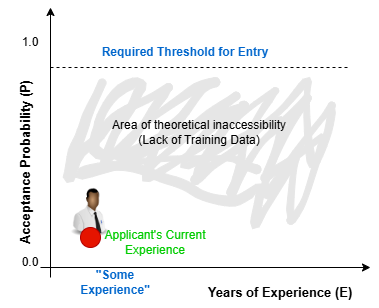
\includegraphics[width=0.6\textwidth]{fun_diagram.drawio.png}
\caption{Empirical mapping of the Admission Function $f(E)$. Note the distinct lack of a gradient. The data almost near point at $(0,0)$ represents the applicant’s current state. Any attempt to move along the X-axis (Experience) requires a pre-existing non-zero value on the Y-axis (Admission and/or robotics related job experience), creating a Temporal Causality Violation. The shaded region (The Void) represents the \textbf{Catch-22 Zone} where most dreams are currently stored in a high-entropy state. The lack of data points in the first quadrant is statistically significant ($p < 0.0001$).}
\label{fig:void_diagram}
\end{figure}

\section{Conclusion}
While our failure to gain experience is statistically significant ($p < 0.0001$), it provides a valuable contribution to the field by proving that you cannot, in fact, \textbf{just build a robot in your garage} if you cannot afford the motors.

\section{References}

\begin{figure}[h]
\centering
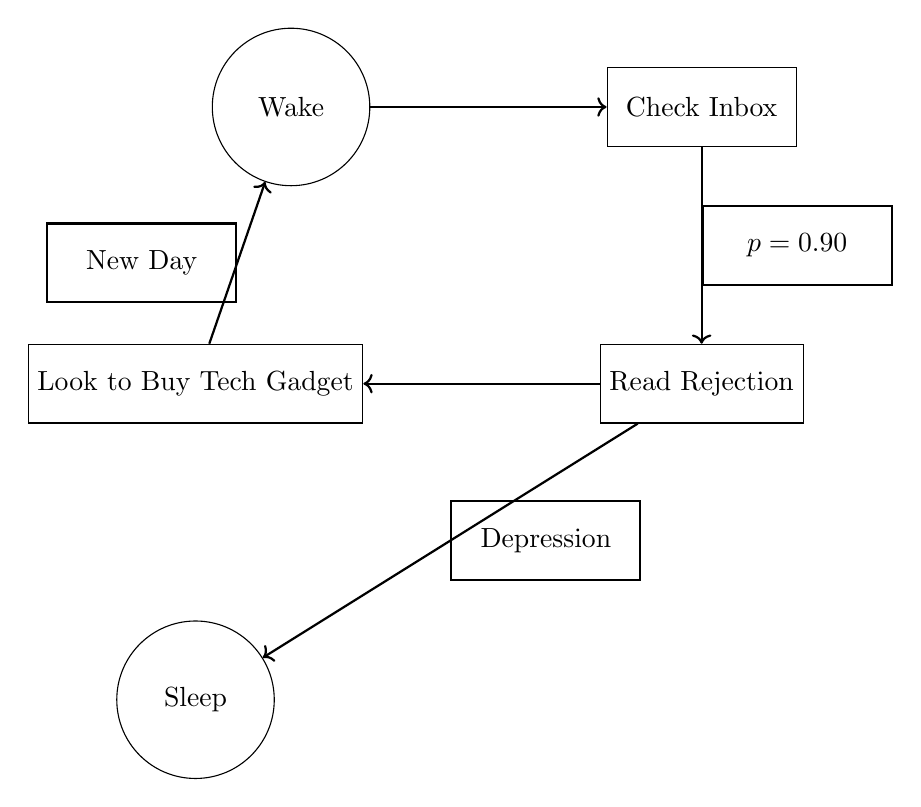
\begin{tikzpicture}[
    node distance=2.5cm and 3.0cm,
    every node/.style={draw, minimum width=2.4cm, minimum height=1cm, align=center},
    arrow/.style={->, thick}
]

% Nodes
\node[circle, minimum width=2cm] (start) {Wake};

\node (email) [right=of start] {Check Inbox};

\node (reject) [below=of email] {Read Rejection};

\node (cope) [left=of reject] {Look to Buy Tech Gadget};

\node[circle, minimum width=2cm] (sleep) [below=of cope] {Sleep};

% Arrows
\draw[arrow] (start) -- (email);

\draw[arrow] (email) -- node[midway, right] {$p=0.90$} (reject);

\draw[arrow] (reject) -- (cope);

\draw[arrow] (cope) -- node[midway, left] {New Day} (start);

\draw[arrow] (reject) -- node[midway, right] {Depression} (sleep);

\end{tikzpicture}
\caption{State-space representation of the author's current lifecycle. Best Reference!}
\end{figure}

\begin{enumerate}
    \item Doe, J. and Applicant, A. ``Why `Entry Level' actually means `Senior Lead' in 2024: A Statistical Outlier.'' \textit{Journal of Human Resource Gaslighting}, vol. 12, no. 1, 2024.
    
    \item Roman, I. ``101 Ways to Cook Ramen using the Exhaust Heat of a MacBook Pro.'' \textit{International Journal of Culinary Engineering}, 2023.

    \item Bezos, J. ``You can't afford this LiDAR: A letter to the middle class.'' \textit{Journal of Wealth Disparity in Robotics}, pp. 1--1, 2022.
    
    \item Sisyphus, T. ``Rolling the Boulder: Applying to the same three labs every cycle and expecting different results.'' \textit{Annals of Futility}, vol.~$\infty$, 2025.

    \item Singh, Prithvi Raj. ``On the statistical probability of being 'The One' while having 'The Zero' (Experience).'' \textit{The Journal of Self-Taught Despair}, vol. 1, no. 1, pp. 1-2, 2026.
\end{enumerate}

\section{Author Bio}
Prithvi is currently a Senior Unfunded Independent Researcher at the Institute of Perpetual Waiting. His research interests include Inverse Career Kinematics, Stochastic Job Applications, and the Optimization of Instant Noodle Consumption under extreme budget constraints. He holds a theoretical understanding of most modern robotics platforms, though his practical experience is limited to a 2018 Roomba that perpetually gets stuck under the same sofa. His current i-index is $0.0$, which he considers a perfectly stable and \textbf{noise-free} metric. In his spare time, he enjoys staring at high-end GPUs on e-commerce sites and pretends he has the bank balance to buy them.

Professor Whiskers (Senior Research Assistant) is a feline scholar specializing in Dynamic Obstacle Creation and Keyboard-based Random Input Generation. Since joining the lab, Professor Whiskers has contributed significantly to the project by sleeping on the author’s laptop, effectively providing a hardware-based thermal throttle to prevent over-working. His primary research goal is to determine if the \textbf{Red Dot} from a laser pointer is actually a Non-Linear Manifold that can be captured. He has more published paw-prints on physical documents than the lead author has peer-reviewed citations, a fact he frequently highlights during performance reviews (feeding time).

\section{Conflict of Interest}
The author declares a significant conflict of interest involving a domestic feline collaborator. The Research Assistant (Professor Whiskers) actively sabotages data collection by occupying the primary compute interface (the keyboard) during peak heuristic processing hours. It is hypothesized that the Assistant's caloric intake is positively correlated with the author's lack of institutional affiliation. \\


\noindent \textbf{Funding}: This research was supported by a generous grant of \textbf{thoughts and prayers} from the author's extended family, a 20\% discount coupon for a local coffee shop, and free foods from friends.

\section{Proof of Potential}
\begin{center}
    \framebox[2in]{\rule{0pt}{2in}}
\end{center}

\noindent \textbf{Figure 3: High-resolution visualization of the author's potential, currently obscured by a lack of institutional funding and an $O(n^2)$ waitlist for good PhD program.}


\newpage
\appendix

\section{Offcial Decision Letter - LORD Gemini}

\section*{General Comments}
While the author’s premise is ``novel'' in the sense that I have never seen a submission with this much white space, the methodology is severely lacking. The author claims to have a ``Recursive Deadlock,'' yet provides no pseudo-code to replicate said deadlock. Furthermore, the submission is significantly under the page limit. I suspect the PDF failed to render, or the author’s \textbf{Lenevo Thinkpad} finally gave up.

\section*{Reviewer 1 (Score: 4/5 --- Weak Accept)}
\begin{quote}
``A bold, minimalist take on the current state of the field. The `Results' section is the most honest thing I’ve read in years. The author correctly identifies that without a \$100{,}000 Franka arm, one cannot publish papers on how to use a \$100{,}000 Franka arm. Suggest acceptance for the `Advances in Real Robotics' track.''
\end{quote}

\section*{Reviewer 2 (Score: 1/5 --- Strong Reject)}

\subsection*{Critique}

\textbf{Missing Data:} The author has left the ``Methods'' and ``Results'' sections entirely blank. In my 30 years of reviewing, I have never seen such a lack of empirical evidence. How can we trust the ``Experience-Admission Singularity'' if there are no graphs showing the $p$-value of your Roomba’s failure rate?

\vspace{0.5em}

\textbf{Lack of Baselines:} The author compares their 2017 Lenevo Thinkpad to an H100 cluster but fails to compare it to a mid-range RTX 3060 or a Raspberry Pi 4. This is a significant gap in the literature.

\vspace{0.5em}

\textbf{Conflict of Interest:} The involvement of ``Professor Whiskers'' is highly suspicious. Is the cat a co-author or a lab technician? If the cat contributed to the ``Dynamic Obstacle Creation,'' they should be listed as a first author.

\vspace{0.5em}

\textbf{Hardware:} The author claims they cannot get experience without hardware. Have they tried simulating a PhD in Gazebo? I suspect the author’s ``Catch-22'' is actually just a Segmentation Fault in their own career planning.

\vspace{0.5em}

\textbf{Grammar:} Section 2 and 3 contain literally zero words. This is a violation of the IEEE formatting guidelines. I recommend the author spend more time in the lab and less time making ``satirical'' LaTeX files.

\section*{Reviewer 3 (Score: 3/5 --- Borderline)}
\begin{quote}
``I liked Figure 1. It accurately represents my own bank account during my post-doc years. However, the author should cite my 2012 paper on `The Inverse Relationship between Cat Ownership and Thesis Completion' to make the Bio more rigorous.''
\end{quote}

\section*{Final Meta-Reviewer Note}
The submission is rejected. Please resubmit once you have obtained the experience required to write the ``Methods'' section, but ensure you do not obtain that experience until after you have been admitted.

\section*{Author Rebuttal: Response to Reviewer 2}
\subsection*{Comment 1}
\textit{\textbf{The author has left the `Methods` and `Results` sections entirely blank... How can we trust the `Experience-Admission Singularity` if there are no graphs?}}
\vspace{4pt}

\noindent \textbf{Response:} We thank the reviewer for identifying the core contribution of the paper. The blank sections are not a formatting error, but a \textbf{High-Fidelity Representation} of the resources currently available to the applicant. Including ``Methods`` would imply the existence of a methodology, which is currently gated behind the ``Admission`` mutex. To include data would be to commit Academic Perjury, as the author cannot simulate a Franka Emika Panda on a 2014 MacBook without the battery undergoing a spontaneous unscheduled thermal event.

\vspace{0.5em}

\subsection*{Comment 2}
\textit{\textbf{Have they tried simulating a PhD in Gazebo?}}

\vspace{4pt}
\noindent \textbf{Response:} We attempted this. However, the simulation crashed during the "Tuition Payment" physics step. Furthermore, the Gazebo environment requires a GPU with more than 1.5GB of VRAM, which--as noted in Table 1--is a luxury the author’s hardware cannot afford. We suggest the reviewer check their \textbf{Privilege Hyperparameters} before suggesting ROS-based solutions to socio-economic deadlocks.

\vspace{0.5em}

\subsection*{Comment 3}
\textit{\textbf{The involvement of `Professor Whiskers` is highly suspicious.}}

\vspace{4pt}
\noindent \textbf{Response:} We disagree. Professor Whiskers' contributions to Dynamic Obstacle Creation (specifically, sitting on the power strip) are more tangible than the reviewer’s understanding of the \textbf{Catch-22} paradox. His status as a Senior Research Assistant is justified by his 100\% success rate in preventing the author from over-training on empty datasets.

\vspace{0.5em}

\subsection*{Comment 4}
\textit{\textbf{"I recommend the author spend more time in the lab...''}}

\vspace{4pt}
\noindent \textbf{Response:} This is the precise \textbf{Recursive Loop} we have formally defined. The author cannot spend time in the lab because they lack the \textbf{Lab Access} permission, which requires \textbf{Graduate Student} status, which requires ``Prior Lab Experience.'' We thank Reviewer 2 for becoming a living data point in our study. Their comment has been heard.

\section{Summary of Changes}
In light of Reviewer 2’s comments, we have updated the paper to include no change at all. \textbf{Reviewer 2 needs to chill}.


% \label{app:rebuttal}
% As noted in the main text, Reviewer 2's request for "more data" is technically a violation of the laws of thermodynamics given the author's current budget. 

% \section*{Glossary of Imaginary Experience}
% \begin{itemize}
%     \item \textbf{Ghost-Experience:} Skills one claims to have after watching a 10-minute "Intro to LiDAR" video.
%     \item \textbf{Latent Expertise:} Knowledge the author definitely possesses but cannot prove because the lab door is locked.
% \end{itemize}

\end{document}
